%\begin{cutout}{2}{0pt}{0.5\linewidth}{13}
\begin{wrapfigure}[16]{R}{0.6\textwidth}
%\begin{figure}[!htb]
\vspace*{-1.5em}
\graphicspath{{figures/trapezoidZ}}
    \centering
    %\subfloat[]{
        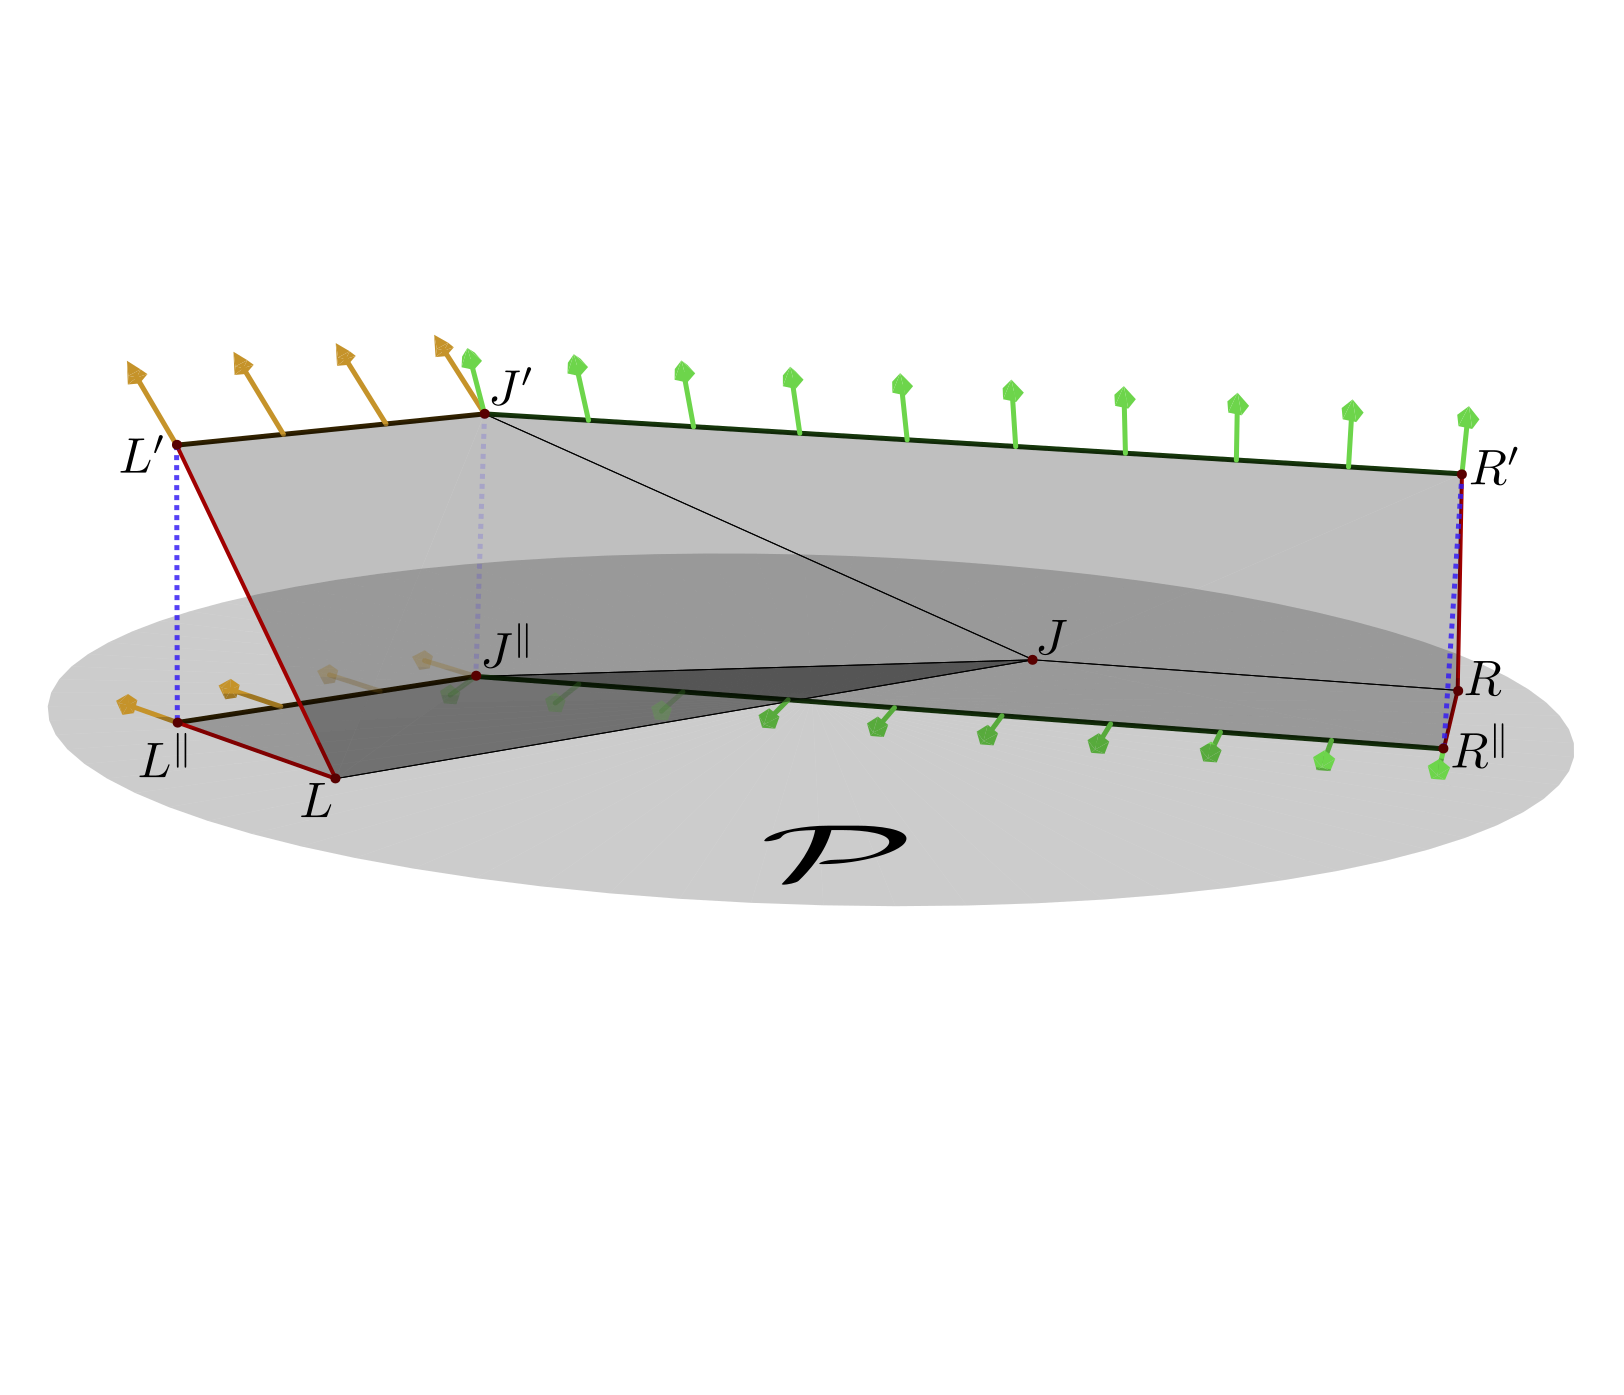
\includegraphics[width=0.35\textwidth]{figures/trapezoidZ/trapezoidZ0.pdf}%
    %}%
    %\subfloat[]{
        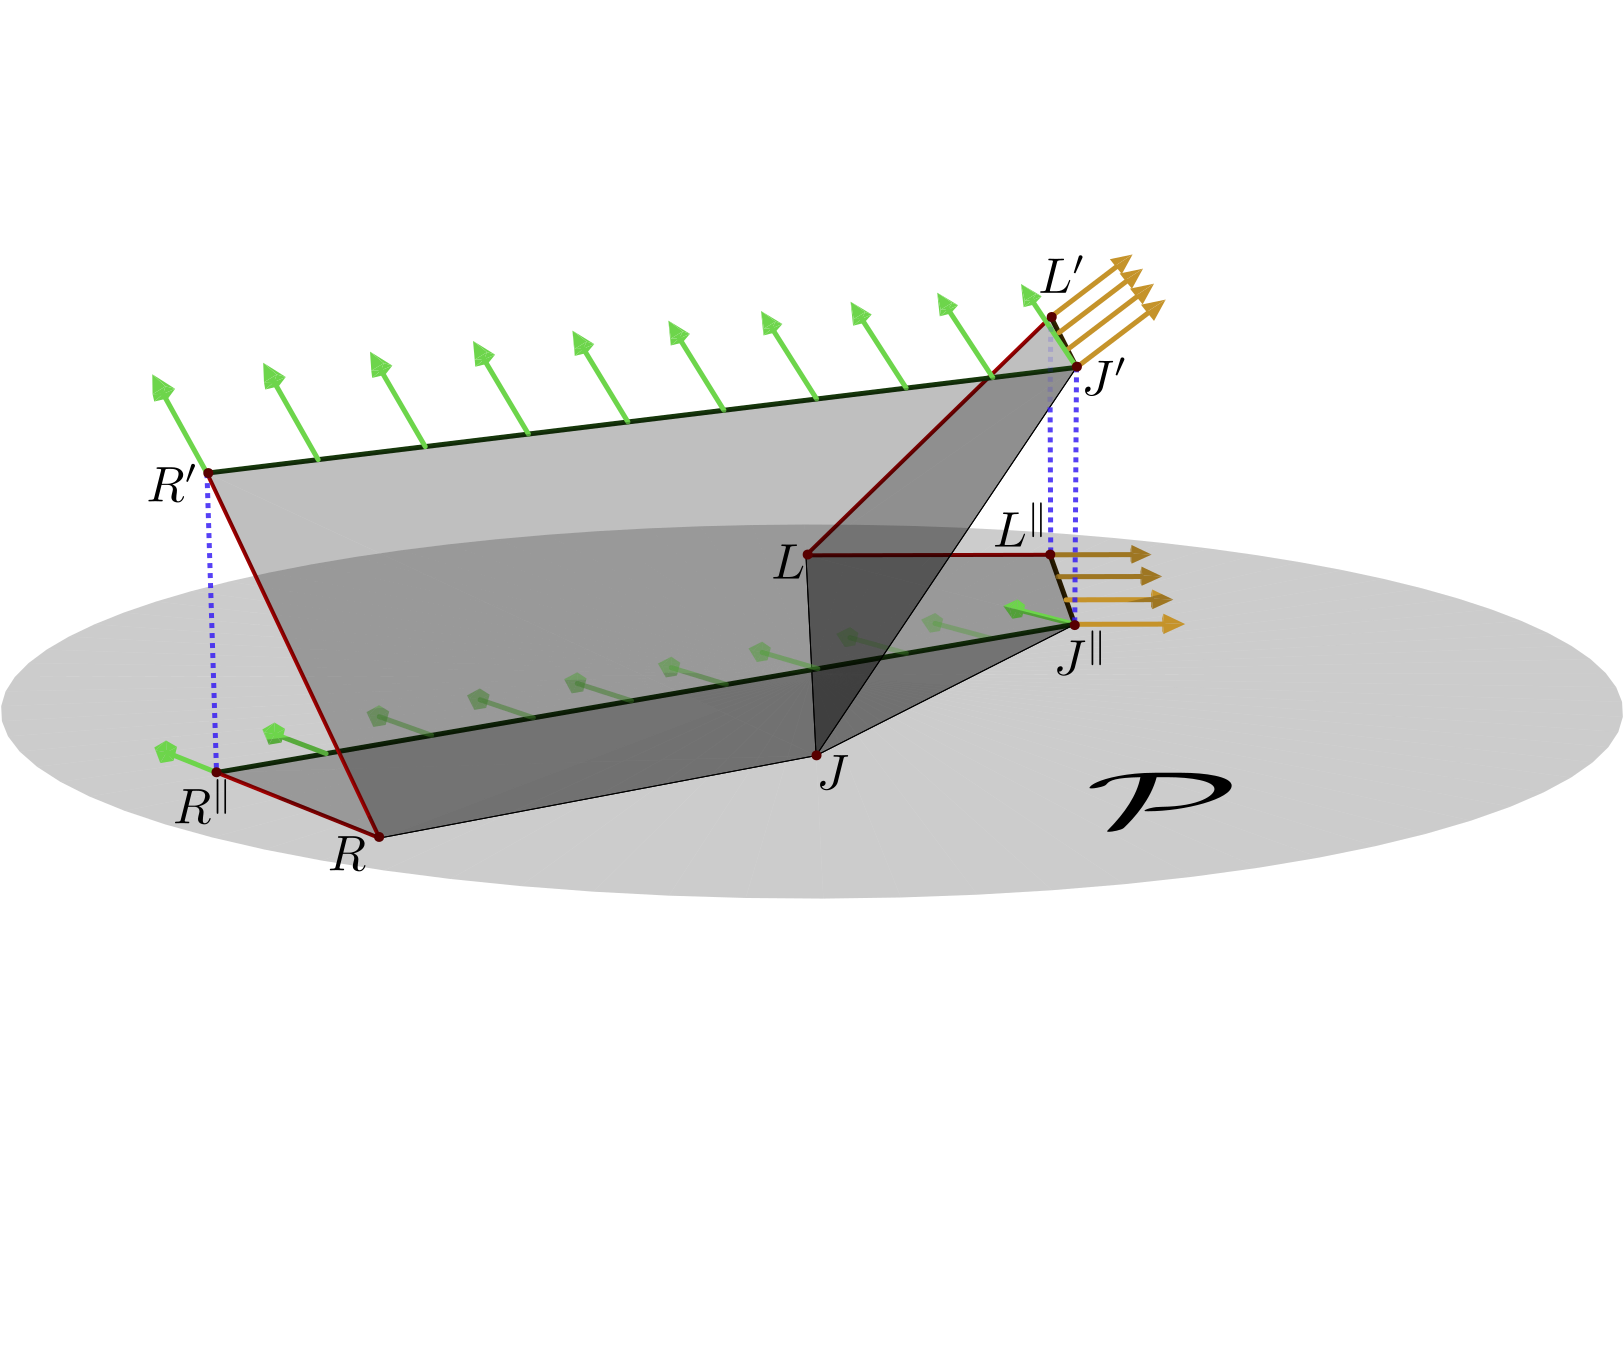
\includegraphics[width=0.35\textwidth]{figures/trapezoidZ/trapezoidZ1.pdf}%
    %}%

    %\subfloat[]{
        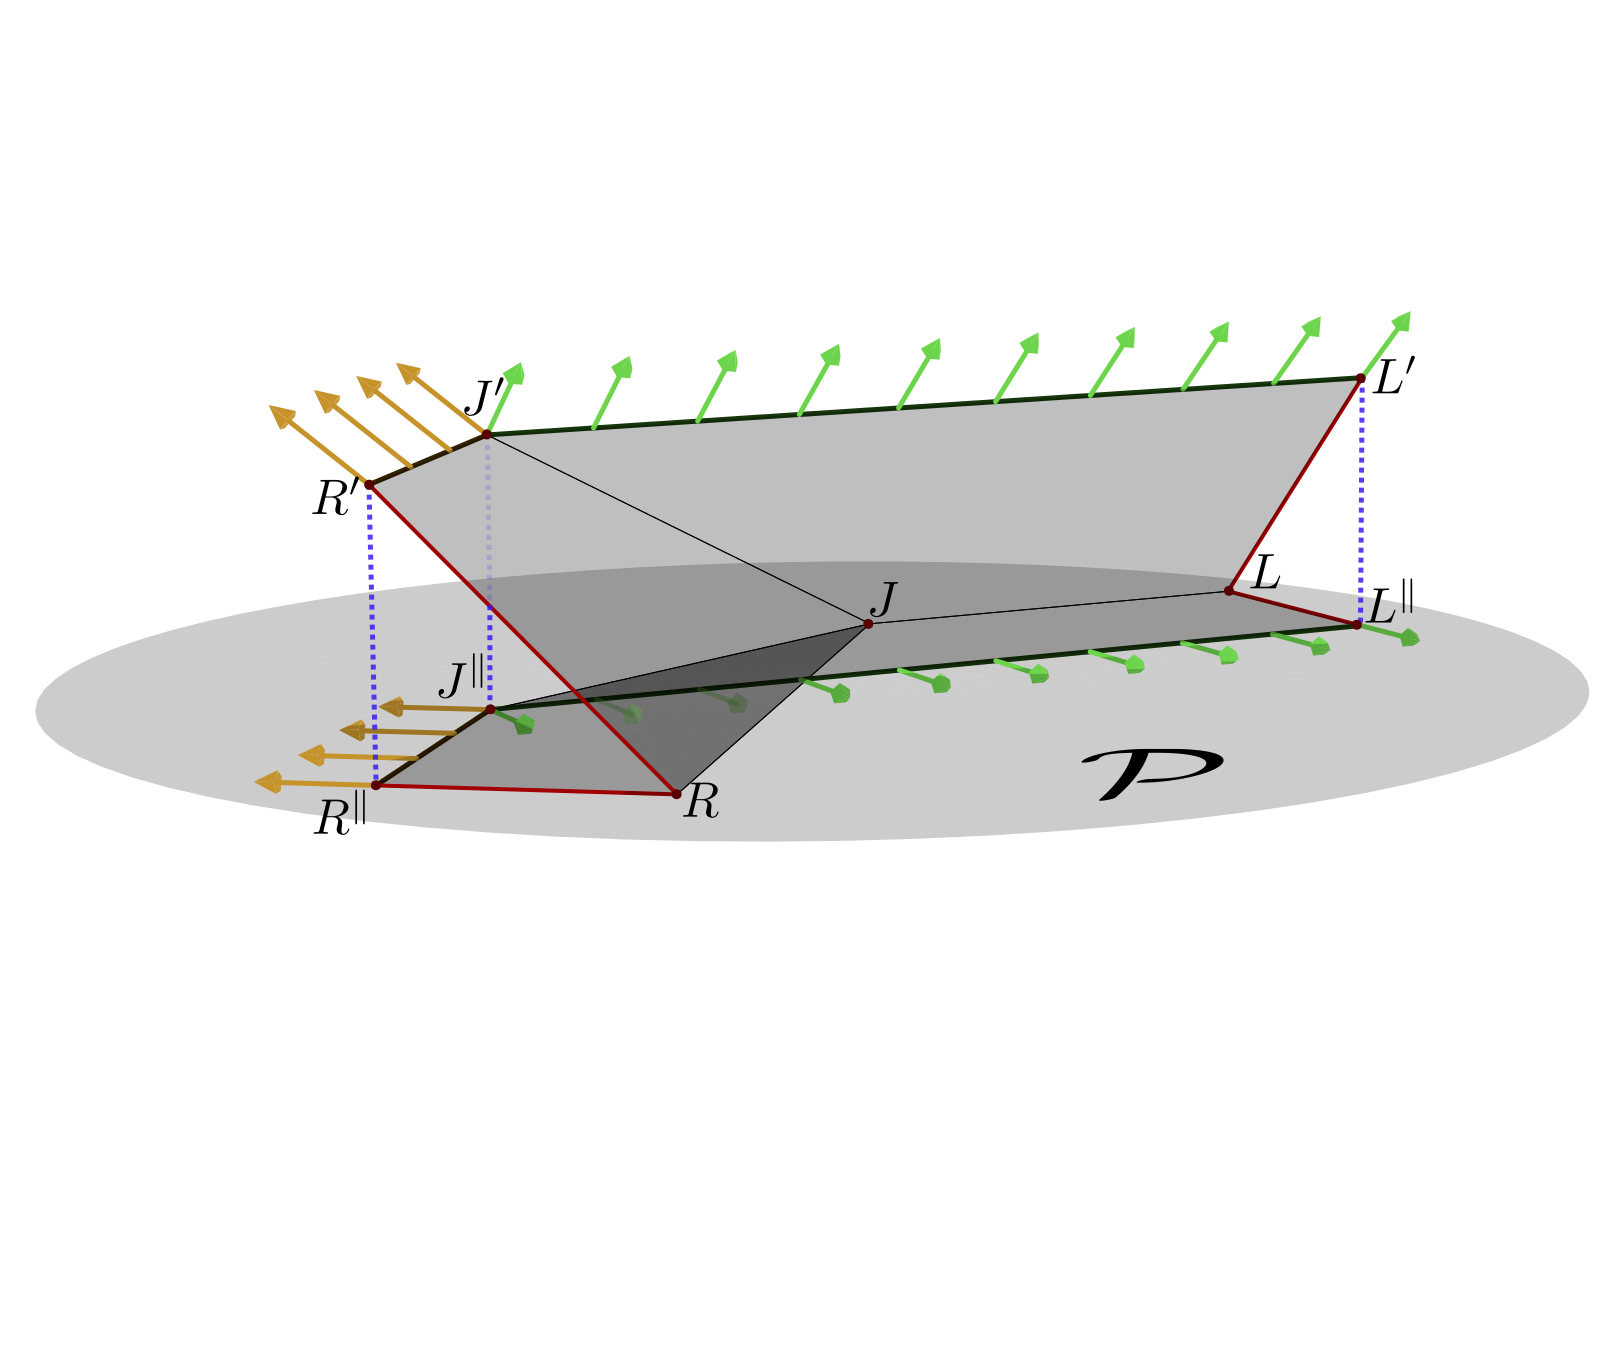
\includegraphics[width=0.7\textwidth]{figures/trapezoidZ/trapezoidZ2.pdf}%
    %}%
    \caption{
    Evolution of a joint with non-zero orthogonal velocity from $LJR$ to $L'J'R'$.
    The blue dotted lines are the projection of the final state to the joint plane $\mathcal P$.
    }
    \label{fig:trapezoidZ}
%\end{figure}
\end{wrapfigure}
%\end{cutout}
